% ====================================================================
% VİZE RAPOR ŞABLONU – Türk Masalları Derlemesi Web Sayfası
% --------------------------------------------------------------------
% DERLEME: Overleaf'te Menu > Compiler > XeLaTeX (pdfLaTeX de çalışır).
%
% KURALLAR (şablonu kullanmadan önce okuyun):
%  1. Bölüm başlıklarını SİLMEYİN ve sırasını DEĞİŞTİRMEYİN.
%  2. [KÖŞELİ PARANTEZ] içindeki ve gri renkli açıklama metinlerini
%     kendi bilgilerinizle değiştirin; açıklama metinlerini silin.
%  3. MEBİS'e YALNIZCA bu raporun PDF'ini yükleyin.
%     ZIP ve HTML dosyası YÜKLEMEYİN. Tüm kontroller GitHub'dan yapılır.
%  4. Kapaktaki GitHub ve YouTube bağlantıları doğru ve tıklanabilir
%     olmalıdır. Teslimden önce PDF'teki bağlantılara tıklayıp deneyin.
%  5. Haftalık katkı tablosundaki görseller için resim dosyalarını
%     (hafta1.png, hafta2.png, ...) Overleaf projesine yükleyin.
%     Dosya adlarında boşluk ve Türkçe karakter kullanmayın.
%     Resim yoksa tabloda "görsel ekleyin" kutusu görünür.
%  6. Yapay zekâ kullandıysanız Bölüm 5'i doldurun.
% ====================================================================
\documentclass[12pt,a4paper]{article}

\usepackage{iftex}
\ifPDFTeX
  \usepackage[T1]{fontenc}
  \usepackage[utf8]{inputenc}
\else
  \usepackage{fontspec}
\fi
\usepackage[turkish]{babel}
\usepackage[margin=2.4cm]{geometry}
\usepackage{setspace}
\usepackage{graphicx}
\usepackage{booktabs}
\usepackage{longtable}
\usepackage{array}
\usepackage{colortbl}
\usepackage{xcolor}
\usepackage{enumitem}
\usepackage{listings}
\usepackage{amssymb}
\usepackage{caption}
\usepackage{fancyhdr}
\usepackage{hyperref}

\onehalfspacing
\setlength{\parindent}{0pt}
\setlength{\parskip}{6pt}
\setlist{itemsep=2pt, topsep=4pt}
\hypersetup{colorlinks=true, linkcolor=blue!50!black, urlcolor=blue!50!black}

\definecolor{ana}{HTML}{14325C}
\definecolor{acik}{HTML}{EEF2F8}

\lstset{basicstyle=\ttfamily\small, backgroundcolor=\color{acik},
  frame=single, rulecolor=\color{ana}, breaklines=true,
  columns=fullflexible, keepspaces=true, showstringspaces=false}

\pagestyle{fancy}
\fancyhf{}
\fancyhead[L]{[PROJE ADI]}
\fancyhead[R]{Vize Raporu}
\fancyfoot[C]{\thepage}

% ---------- Yardımcı komutlar ----------
% Gri açıklama metni (silinecek yönergeler için)
\newcommand{\aciklama}[1]{{\color{gray}\itshape (#1)}}

% Haftalık tablo görseli: dosya yoksa "görsel ekleyin" kutusu çıkar
\newcommand{\haftagorsel}[1]{%
  \IfFileExists{#1}{%
    \includegraphics[width=\linewidth,height=4.2cm,keepaspectratio]{#1}%
  }{%
    \fbox{\parbox[c][2.6cm][c]{\dimexpr\linewidth-2\fboxsep-2\fboxrule\relax}{%
      \centering\small\color{gray} Ekran görüntüsü / görsel ekleyin\\ \texttt{#1}}}%
  }%
}
% Haftalık katılım kutuları (işaretlemek için $\square$ yerine $\boxtimes$ yazın)
\newcommand{\katilimkutulari}{\par\vspace{3pt}\small $\square$ Ders içinde katılım sergiledim\par $\square$ Telafi yaptım}

% Ek görsel: dosya yoksa hiçbir şey göstermez
\newcommand{\haftaek}[1]{%
  \IfFileExists{#1}{\\[4pt]\includegraphics[width=\linewidth,height=4.2cm,keepaspectratio]{#1}}{}%
}

% ---------- Kapak bilgileri ----------
\newcommand{\universite}{[ÜNİVERSİTE / BÖLÜM]}
\newcommand{\dersadi}{[DERS ADI]}
\newcommand{\hocaadi}{[ÖĞRETİM ÜYESİ]}
\newcommand{\ogrenciadi}{[AD SOYAD]}
\newcommand{\ogrencino}{[ÖĞRENCİ NUMARASI]}
\newcommand{\projeadi}{[PROJE ADI]}
% Bağlantıları tam adres olarak yazın (https:// ile başlayarak)
\newcommand{\githublink}{\url{https://github.com/KULLANICI-ADI/DEPO-ADI}}
\newcommand{\youtubelink}{\url{https://www.youtube.com/watch?v=VIDEO-KIMLIGI}}

\begin{document}

% ====================================================================
% KAPAK
% ====================================================================
\begin{titlepage}
\centering
\vspace*{1cm}
{\large \universite \par}
\vspace{1.8cm}
{\Huge\bfseries\color{ana} \projeadi \par}
\vspace{0.4cm}
{\Large Türk Masalları Derlemesi Web Sayfası \par}
{\large Vize Raporu \par}
\vspace{1.8cm}
{\large \textbf{Ders:} \dersadi \par}
{\large \textbf{Öğretim Üyesi:} \hocaadi \par}
\vspace{1.2cm}
{\large \textbf{Hazırlayan:} \ogrenciadi \par}
{\large \textbf{Öğrenci No:} \ogrencino \par}
\vspace{1.8cm}
\fbox{\parbox{0.88\linewidth}{\centering\vspace{6pt}
{\large\bfseries Proje Bağlantıları}\\[8pt]
\textbf{GitHub deposu:}\\ \githublink \\[8pt]
\textbf{YouTube sunum videosu:}\\ \youtubelink
\vspace{6pt}}}
\vfill
{\large \today \par}
\end{titlepage}

\tableofcontents
\newpage

% ====================================================================
\section{Giriş}
% ====================================================================
\aciklama{Projenin amacını, neyi neden yaptığınızı ve raporun içeriğini 5--8 cümleyle
anlatın. Ödev gereksinimlerini (8--12 masal, tek HTML dosyası, içsel CSS ve içsel
JavaScript) nasıl karşıladığınızı belirtin.}

\subsection{Proje Özeti}
[Projenizin kısa özeti.]

\subsection{Gereksinimlerin Karşılanması}
\begin{center}
\rowcolors{2}{acik}{white}
\begin{tabular}{@{}p{8.2cm}c@{}}
\toprule
\rowcolor{ana}\textcolor{white}{\textbf{Gereksinim}} & \textcolor{white}{\textbf{Durum}} \\
\midrule
Masal sayısı 8--12 arasında ([SAYI] masal)         & $\square$ \\
Tek HTML dosyası                                    & $\square$ \\
Stil kodları içsel (\texttt{<style>} içinde)        & $\square$ \\
Betik kodları içsel (\texttt{<script>} içinde)      & $\square$ \\
İnternetsiz açılıp çalışıyor                        & $\square$ \\
JavaScript sayfada anlamlı bir işlev görüyor        & $\square$ \\
Masal metinleri kendi cümlelerimle yazıldı          & $\square$ \\
Sayfa telefonda da düzgün görünüyor                 & $\square$ \\
\bottomrule
\end{tabular}
\end{center}
\aciklama{Karşıladığınız her satırın kutusunu $\boxtimes$ ile değiştirin.}

% ====================================================================
\section{Masalların Seçimi}
% ====================================================================
\aciklama{Hangi masalları, hangi ölçütlere göre seçtiniz? Tabloyu masal sayınıza göre
düzenleyin (en az 8, en fazla 12 satır). Kullandığınız kaynakları Kaynakça'ya yazın.}

\begin{longtable}{@{}cp{4cm}p{3cm}p{5.4cm}@{}}
\toprule
\textbf{No} & \textbf{Masal} & \textbf{Tür} & \textbf{Seçilme nedeni} \\
\midrule
\endhead
1 & [Masal adı] & [Tür] & [Neden seçtiniz?] \\
2 & [Masal adı] & [Tür] & [Neden seçtiniz?] \\
3 & [Masal adı] & [Tür] & [Neden seçtiniz?] \\
4 & [Masal adı] & [Tür] & [Neden seçtiniz?] \\
5 & [Masal adı] & [Tür] & [Neden seçtiniz?] \\
6 & [Masal adı] & [Tür] & [Neden seçtiniz?] \\
7 & [Masal adı] & [Tür] & [Neden seçtiniz?] \\
8 & [Masal adı] & [Tür] & [Neden seçtiniz?] \\
9 & [Masal adı] & [Tür] & [Neden seçtiniz?] \\
10 & [Masal adı] & [Tür] & [Neden seçtiniz?] \\
\bottomrule
\end{longtable}

% ====================================================================
\section{Tasarım Kararları}
% ====================================================================
\aciklama{Tasarım size aittir; hazır taslak (şablon) kullanılmamıştır. Burada
tasarımınızın masal okuma amacına nasıl hizmet ettiğini gerekçeleriyle anlatın.}

\subsection{Konuya Uygunluk}
[Renk, yazı tipi ve görsellerin Türk masalı temasıyla bağlantısını ve nedenlerini yazın.]

\subsection{Renk Paleti ve Yazı Tipi}
\begin{center}
\rowcolors{2}{acik}{white}
\begin{tabular}{@{}llp{6.4cm}@{}}
\toprule
\rowcolor{ana}\textcolor{white}{\textbf{Ad}} & \textcolor{white}{\textbf{Kod}} & \textcolor{white}{\textbf{Nerede / neden kullandınız?}} \\
\midrule
\relax[Renk adı] & \texttt{[\#HEX]} & [Kullanım ve gerekçe] \\
\relax[Renk adı] & \texttt{[\#HEX]} & [Kullanım ve gerekçe] \\
\relax[Renk adı] & \texttt{[\#HEX]} & [Kullanım ve gerekçe] \\
\relax[Yazı tipi] & -- & [Başlık ve metin için seçim gerekçesi] \\
\bottomrule
\end{tabular}
\end{center}

\subsection{Okunabilirlik, Gezinme ve Duyarlı Tasarım}
\begin{itemize}
  \item \textbf{Okunabilirlik:} [Yazı boyutu, satır uzunluğu, zemin--metin karşıtlığı.]
  \item \textbf{Gezinme:} [Kullanıcı istediği masala nasıl ulaşıyor?]
  \item \textbf{Duyarlı tasarım:} [Telefon ve bilgisayarda düzen nasıl değişiyor?]
  \item \textbf{Tutarlılık:} [Başlık, boşluk ve renklerin kullanımı.]
\end{itemize}

\subsection{Ekran Görüntüleri}
\aciklama{Aşağıdaki satırların başındaki \% işaretini kaldırıp dosya adlarını kendi
görsellerinizle değiştirin.}
% \begin{figure}[h]
%   \centering
%   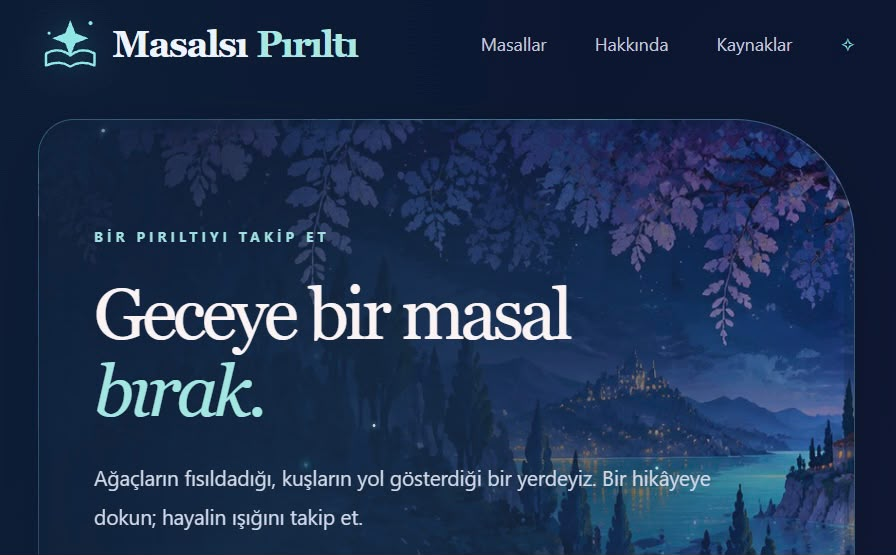
\includegraphics[width=0.9\textwidth]{ekran-masaustu.png}
%   \caption{Sayfanın bilgisayar görünümü}
% \end{figure}
% \begin{figure}[h]
%   \centering
%   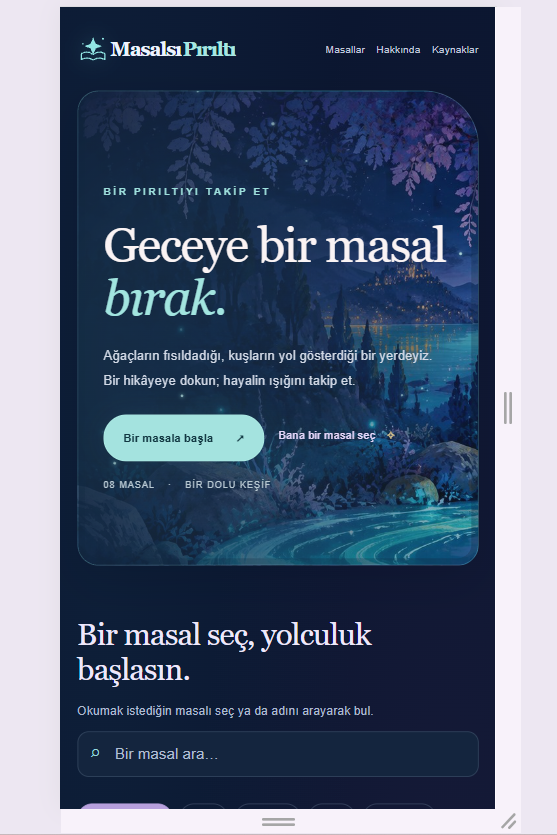
\includegraphics[width=0.35\textwidth]{ekran-mobil.png}
%   \caption{Sayfanın telefon görünümü}
% \end{figure}

% ====================================================================
\section{Gerçekleştirme}
% ====================================================================
\aciklama{Sayfanın nasıl çalıştığını kendi cümlelerinizle anlatın. Kodu sunumda
açıklayabilmelisiniz; burada da mantığını yazın. Kodun tamamını değil, önemli
bölümlerini kısa örneklerle gösterin.}

\subsection{HTML Yapısı}
[Sayfanın bölümleri (başlık, liste, okuma alanı, alt bilgi vb.) ve kullandığınız etiketler.]

\subsection{İçsel CSS}
[Önemli stil kararları: değişkenler, düzen (grid/flex), duyarlı tasarım kuralları.]

\begin{lstlisting}[caption={İçsel CSS'ten önemli bir bölüm}]
/* Kendi kodunuzdan kısa bir örnek yapıştırın.
   Türkçe karakterlerden kaçının veya açıklamaları ASCII yazın. */
\end{lstlisting}

\subsection{İçsel JavaScript}
[Masal verisi nasıl tutuluyor? Hangi fonksiyonlar ne yapıyor? Olaylar nasıl bağlanıyor?]

\begin{lstlisting}[caption={İçsel JavaScript'ten önemli bir bölüm}]
// Kendi kodunuzdan kısa bir örnek yapıştırın.
\end{lstlisting}

\subsection{Sayfanın Özellikleri}


% ====================================================================
\section{Yapay Zekâ Kullanımı}
% ====================================================================
\aciklama{Yapay zekâ kullanımı kod ve görsel için serbesttir; koşul, çalışmanın mantığını
anlatabilmenizdir. Kullandığınız araçları aşağıya yazın. Hiç kullanmadıysanız tek
satırda ``Yapay zekâ aracı kullanılmamıştır'' yazın ve tabloyu silin.}

\begin{longtable}{@{}p{2.6cm}p{3.6cm}p{4.2cm}p{3.4cm}@{}}
\toprule
\textbf{Araç} & \textbf{Ne için kullandınız?} & \textbf{İstem (prompt) özeti} & \textbf{Sayfada nerede?} \\
\midrule
\endhead
\relax[Araç adı] & [Kod / görsel / metin] & [Kısa özet] & [Bölüm veya görsel] \\
\relax[Araç adı] & [Kod / görsel / metin] & [Kısa özet] & [Bölüm veya görsel] \\
\bottomrule
\end{longtable}

\subsection{Anladığım ve Kendim Yaptığım Kısımlar}
jfjfjfjfjfjfjfjfjfjfjjfjffjjfjfjffjfjfj

% ====================================================================
\section{Haftalık Katkılar}
% ====================================================================
\aciklama{Her hafta ders içinde yaptığınız çalışmayı kısaca yazın (2--4 cümle). Hangi
özelliği eklediğinizi ya da neyi düzelttiğinizi belirtin ve ilgili commit mesajını
ya da bağlantısını ``Commit'' satırına yazın. Her satıra ekran görüntüsü ekleyin:
resimleri \texttt{hafta1.png}, \texttt{hafta2.png}, \ldots{} adıyla Overleaf
projesine yükleyin. Aynı haftaya ikinci bir görsel eklemek için
\texttt{hafta1b.png} gibi bir dosya yükleyin; kendiliğinden görünür.
Her haftanın altındaki kutulardan o hafta için geçerli olanı $\boxtimes$ ile
işaretleyin: dersin kendisinde katılım gösterdiyseniz ``Ders içinde katılım
sergiledim'', o haftayı sonradan tamamladıysanız ``Telafi yaptım''. Telafi
yaptıysanız yapılan çalışmanın metninde bunu açıkça belirtin.}

\begin{longtable}{@{}>{\raggedright\arraybackslash}p{1.7cm}%
                    >{\raggedright\arraybackslash}p{6.4cm}%
                    >{\centering\arraybackslash}p{6cm}@{}}
\toprule
\rowcolor{ana}\textcolor{white}{\textbf{Hafta}} & \textcolor{white}{\textbf{Yapılan çalışma}} & \textcolor{white}{\textbf{Görsel}} \\
\midrule
\endfirsthead
\toprule
\rowcolor{ana}\textcolor{white}{\textbf{Hafta}} & \textcolor{white}{\textbf{Yapılan çalışma}} & \textcolor{white}{\textbf{Görsel}} \\
\midrule
\endhead
\bottomrule
\endfoot

\textbf{1. hafta}\newline [tarih] &
[Bu hafta yaptığınız çalışma.]\newline \textbf{Commit:} [mesaj veya bağlantı]\katilimkutulari &
\haftagorsel{hafta1.png}\haftaek{hafta1b.png} \\
\midrule
\textbf{2. hafta}\newline [tarih] &
[Bu hafta yaptığınız çalışma.]\newline \textbf{Commit:} [mesaj veya bağlantı]\katilimkutulari &
\haftagorsel{hafta2.png}\haftaek{hafta2b.png} \\
\midrule
\textbf{3. hafta}\newline [tarih] &
[Bu hafta yaptığınız çalışma.]\newline \textbf{Commit:} [mesaj veya bağlantı]\katilimkutulari &
\haftagorsel{hafta3.png}\haftaek{hafta3b.png} \\
\midrule
\textbf{4. hafta}\newline [tarih] &
[Bu hafta yaptığınız çalışma.]\newline \textbf{Commit:} [mesaj veya bağlantı]\katilimkutulari &
\haftagorsel{hafta4.png}\haftaek{hafta4b.png} \\
\midrule
\textbf{5. hafta}\newline [tarih] &
[Bu hafta yaptığınız çalışma.]\newline \textbf{Commit:} [mesaj veya bağlantı]\katilimkutulari &
\haftagorsel{hafta5.png}\haftaek{hafta5b.png} \\
\midrule
\textbf{6. hafta}\newline [tarih] &
[Bu hafta yaptığınız çalışma.]\newline \textbf{Commit:} [mesaj veya bağlantı]\katilimkutulari &
\haftagorsel{hafta6.png}\haftaek{hafta6b.png} \\
\midrule
\textbf{7. hafta}\newline [tarih] &
[Bu hafta yaptığınız çalışma.]\newline \textbf{Commit:} [mesaj veya bağlantı]\katilimkutulari &
\haftagorsel{hafta7.png}\haftaek{hafta7b.png} \\
\midrule
\textbf{8. hafta}\newline [tarih] &
[Bu hafta yaptığınız çalışma.]\newline \textbf{Commit:} [mesaj veya bağlantı]\katilimkutulari &
\haftagorsel{hafta8.png}\haftaek{hafta8b.png} \\
\end{longtable}

% ====================================================================
\section{Test ve Değerlendirme}
% ====================================================================
\aciklama{Sayfayı hangi tarayıcı ve cihazlarda denediniz? Çalışmayan bir özellik
olduysa dürüstçe yazın ve nedenini açıklayın.}

\begin{center}
\rowcolors{2}{acik}{white}
\begin{tabular}{@{}p{6cm}p{3.4cm}p{3.4cm}@{}}
\toprule
\rowcolor{ana}\textcolor{white}{\textbf{Özellik}} & \textcolor{white}{\textbf{Bilgisayar}} & \textcolor{white}{\textbf{Telefon}} \\
\midrule
\relax[Özellik 1] & [Çalışıyor / Sorun var] & [Çalışıyor / Sorun var] \\
\relax[Özellik 2] & [Çalışıyor / Sorun var] & [Çalışıyor / Sorun var] \\
\relax[Özellik 3] & [Çalışıyor / Sorun var] & [Çalışıyor / Sorun var] \\
\bottomrule
\end{tabular}
\end{center}

\textbf{Denenen tarayıcılar:} [Chrome, Firefox, Edge, Safari vb.]

% ====================================================================
\section{Sunum Videosu}
% ====================================================================
\begin{center}
\begin{tabular}{@{}ll@{}}
\textbf{Video süresi:} & [dakika:saniye] \quad \aciklama{12--18 dakika olmalıdır} \\
\textbf{Görünürlük:} & [Listelenmemiş / Herkese açık] \\
\textbf{Bağlantı:} & \youtubelink \\
\end{tabular}
\end{center}

\subsection{Video Kontrol Listesi}
\aciklama{Teslimden önce hepsini kontrol edin ve kutuları $\boxtimes$ ile işaretleyin.}
\begin{itemize}[label={}]
  \item $\square$ Süre 12--18 dakika aralığında.
  \item $\square$ Sunum boyunca kameram açık, yüzüm görünüyor.
  \item $\square$ Görünürlük \textbf{Listelenmemiş} (ya da Herkese açık); \textbf{Özel} değil.
  \item $\square$ Bağlantıyı gizli pencerede açtım, video oynuyor.
  \item $\square$ YouTube videoyu işlemeyi bitirdi.
  \item $\square$ Videoyu baştan sona izledim; ses ve kamera tüm sunumda var.
  \item $\square$ Kapaktaki bağlantı ile bu bölümdeki bağlantı aynı.
\end{itemize}

% ====================================================================
\section{Sonuç ve Kendi Değerlendirmem}
% ====================================================================
\aciklama{Projeden ne öğrendiniz? En çok nerede zorlandınız ve nasıl çözdünüz? İleride
neyi geliştirirdiniz? 6--10 cümle yeterlidir.}

[Sonuç metni.]

% ====================================================================
\section{Kaynakça}
% ====================================================================
\aciklama{Masal metinleri için yararlandığınız kitap ve sitelerle, teknik kaynakları
(MDN vb.) ve kullandığınız görsel kaynaklarını yazın. Masalları kendi
cümlelerinizle yazmanız gerekir; kaynaklar yalnızca yararlandığınız yerleri
gösterir.}

\begin{thebibliography}{9}
\bibitem{k1} [Yazar. (Yıl). \emph{Kitap adı}. Yayınevi, Yer.]
\bibitem{k2} [Site adı. \emph{Sayfa başlığı}. Bağlantı, erişim tarihi.]
\end{thebibliography}

% ====================================================================
\appendix
\section{Teslim Kontrol Listesi}
% ====================================================================
\aciklama{Teslim etmeden önce işaretleyin. Bu sayfayı teslim edilen PDF'te bırakabilirsiniz.}
\begin{itemize}[label={}]
  \item $\square$ MEBİS'e \textbf{yalnızca bu raporun PDF'ini} yükleyeceğim. ZIP ve HTML dosyası yüklemeyeceğim.
  \item $\square$ PDF dosya adı \texttt{OgrenciNo\_AdSoyad\_vize.pdf} biçiminde.
  \item $\square$ Kapaktaki GitHub ve YouTube bağlantıları doğru; PDF'te tıklayıp denedim.
  \item $\square$ GitHub deposunda web sayfası (tek \texttt{.html}), rapor PDF'i, \texttt{.tex} kaynakları ve \texttt{README.md} var.
  \item $\square$ GitHub deposu \textbf{herkese açık} (ya da öğretim üyesine erişim verdim).
  \item $\square$ Çalışmamın son hâli teslim saatinden \textbf{önce} depoya gönderildi (sonraki commitler değerlendirilmez).
  \item $\square$ Sayfa içsel CSS ve içsel JavaScript kullanıyor, harici dosya gerektirmiyor.
  \item $\square$ Hazır taslak kullanmadım; yapay zekâ kullandıysam Bölüm 5'i doldurdum.
  \item $\square$ Çalışmanın mantığını sunumda anlatabilirim.
\end{itemize}

\end{document}